\chapter{Numeryczny rozmyty regulator predykcyjny FGPC--SL}
\section{Algorytm z kolejną linearyzacją i ograniczenia}
W części~3 zaimplementowano numeryczny rozmyty regulator predykcyjny z kolejną linearyzacją w bieżącym punkcie pracy -- algorytm FGPC--SL, zgodnie z materiałami wykładowymi \emph{Regulatory rozmyte}, s.~162--163, wzory (4.103)--(4.105) oraz (4.107). Wykorzystuje on dostrojony pięcioregułowy dyskretny model Takagiego--Sugeno wyznaczony w rozdziale~4.

W każdej chwili próbkowania $k$ regulator wyznacza z bieżącego pomiaru poziomu $y(k)=h_2(k)$ znormalizowane wagi reguł $\widetilde w_i(y(k))$ i uśrednia parametry lokalnych równań różnicowych, uzyskując quasi-liniowy model lokalny (wzór (4.107)):
\begin{align}
 \widetilde b_m(k)&=\sum_{i=1}^5\widetilde w_i\bigl(y(k)\bigr)\,b_{m,i},\qquad
 \widetilde c_m(k)=\sum_{i=1}^5\widetilde w_i\bigl(y(k)\bigr)\,c_{m,i}\quad(m=1,2),\\
 \widetilde a_0(k)&=\sum_{i=1}^5\widetilde w_i\bigl(y(k)\bigr)\,a_{0,i}.
\end{align}
Wagi i parametry tego modelu pozostają zamrożone na całym horyzoncie bieżącej predykcji $p=1,\dots,N$. Z bieżącego równania różnicowego wyznaczana jest odpowiedź skokowa $\widetilde s_p(k)$ (z dziesięcioma początkowymi próbkami zerowymi wynikającymi z opóźnienia $\tau=200\ \mathrm{s}$), która buduje macierz dynamiczną $M_k\in\mathbb R^{N\times N_u}$ o elementach $(M_k)_{pj}=\widetilde s_{p-j+1}(k)$ dla $p\geq j$ i zero dla $p<j$.

Trajektorię swobodną $Y^0(k)=[y^0(k+1|k),\dots,y^0(k+N|k)]^{\mathsf T}$ (dla zerowych przyszłych przyrostów sterowania, tj. $u^0(k+j)=u(k-1)$ dla $j\geq0$) wyznacza się rekurencyjnie z zamrożonego modelu liniowego z addytywną korekcją niezmierzonego zakłócenia i niedokładności modelu $d_k$:
\begin{align}
 y^{\mathrm{mod}}(k)&=\widetilde b_1(k)y(k-1)+\widetilde b_2(k)y(k-2)+\widetilde c_1(k)u(k-11)+\widetilde c_2(k)u(k-12)+\widetilde a_0(k),\\
 d_k&=y(k)-y^{\mathrm{mod}}(k),\\
 y^0(k+p|k)&=\widetilde b_1(k)y^0(k+p-1|k)+\widetilde b_2(k)y^0(k+p-2|k)\nonumber\\
 &\quad+\widetilde c_1(k)u^0(k+p-11)+\widetilde c_2(k)u^0(k+p-12)+\widetilde a_0(k)+d_k,
\end{align}
przy warunkach początkowych $y^0(k|k)=y(k)$ i $y^0(k-1|k)=y(k-1)$. W każdej próbce funkcja \texttt{quadprog} rozwiązuje zadanie optymalizacji kwadratowej (wzory (4.103)--(4.105)):
\begin{align}
 \min_{\Delta U}\quad J&=\lVert Y_{\mathrm{zad}}(k)-Y^0(k)-M_k\Delta U\rVert_2^2
                         +\lambda\lVert\Delta U\rVert_2^2,\\
 -15\mathbf 1\leq\Delta U&\leq15\mathbf 1,\qquad
 0\mathbf 1\leq u(k-1)\mathbf 1+L\Delta U\leq200\mathbf 1,
\end{align}
gdzie $\Delta U=[\Delta u(k),\dots,\Delta u(k+N_u-1)]^{\mathsf T}$, $L$ jest dolnotrójkątną macierzą jedynek sumującą przyrosty, a $Y_{\mathrm{zad}}(k)=h_{2,\mathrm{zad}}(k)\mathbf 1$ bez dodatkowego filtrowania wartości zadanej. Ograniczenia w $\jednprzep$ są identyczne jak w rozdziale~5 i dotyczą całego horyzontu sterowania $N_u$. Do obiektu podawany jest pierwszy obliczony przyrost $\Delta u(k)$, po czym procedura powtarza się w następnej próbce.

\section{Strojenie parametru \texorpdfstring{$\lambda$}{lambda} i porównanie z PDC}
Dla regulatora FGPC--SL przyjęto horyzont predykcji $N=30$ ($600\ \mathrm{s}$, tj. 20 próbek za opóźnieniem transportowym) i horyzont sterowania $N_u=5$. Zgodnie z metodyką strojenia ze skryptu (Przykład~4.18, rys.~4.42--4.43) zbadano wpływ współczynnika kary $\lambda\in\{2;\ 1;\ \num{0.5};\ \num{0.2}\}$ na jakość regulacji i charakter sygnału sterującego. Wszystkie próby przeprowadzono na tym samym obiekcie nieliniowym i osi czasu co w częściach~1 i 2 (skok zadania w $400\ \mathrm{s}$, skok $F_D$ w $3800\ \mathrm{s}$, koniec w $8000\ \mathrm{s}$).

\begin{table}[H]
\centering
\caption{Łączny IAE zadania i zakłócenia w czterech próbach projektowych [cm$\cdot$s]: PDC (cz.~2) oraz FGPC--SL ($N=30$, $N_u=5$).}
\small
\begin{tabular}{lrrrrrr}\toprule
$\Delta h_{2,\mathrm{zad}}$ / $\Delta F_D$ & PDC & PDC str. & SL ($\lambda=2$) & SL ($\lambda=1$) & SL ($\lambda=\num{0.5}$) & SL ($\lambda=\num{0.2}$)\\\midrule
$+2\ \mathrm{cm}/+10\ \jednprzep$ & 1746 & 1573 & 1728 & 1522 & 1403 & 1294\\
$+4\ \mathrm{cm}/+20\ \jednprzep$ & 3809 & 3392 & 3541 & 3098 & 2857 & 2646\\
$+8\ \mathrm{cm}/+30\ \jednprzep$ & 7529 & 7001 & 7066 & 5973 & 5343 & 4899\\
$-8\ \mathrm{cm}/-10\ \jednprzep$ & 3187 & 3159 & 4729 & 4232 & 3957 & 3735\\\midrule
Suma & 16271 & 15125 & 17064 & 14823 & 13561 & 12574\\\bottomrule
\end{tabular}
\label{tab:sl-control}
\end{table}

Tab.~\ref{tab:sl-metrics} rozdziela błędy całkowite po skoku zadania i zakłócenia oraz podaje łączną aktywność sterowania $\sum|\Delta u|$, maksymalny ruch $\max|\Delta u|$, maksymalne cofnięcie na dojściu do zadania, maksymalne przeregulowanie oraz maksymalny uchyb po skoku zakłócenia $F_D$.

\begin{table}[H]
\centering
\caption{Wskaźniki jakości regulacji i aktywności sterowania w czterech próbach projektowych.}
\small
\begin{tabular}{lrrrrrrr}\toprule
Regulator & IAE zad. & IAE zakł. & $\sum|\Delta u|$ & $\max|\Delta u|$ & Cofn. & Przereg. & $\max|e_{F_D}|$\\
 & [cm$\cdot$s] & [cm$\cdot$s] & [$\jednprzep$] & [$\jednprzep$] & [cm] & [cm] & [cm]\\\midrule
PDC                       &  9383 & 6888 & \num{490.6} & \num{15.0} & \num{1.296} & \num{0.232} & \num{4.364}\\
PDC strojony              &  8675 & 6450 & \num{459.6} & \num{15.0} & \num{1.019} & \num{0.473} & \num{4.399}\\
FGPC--SL ($\lambda=2$)    & 11963 & 5102 & \num{221.6} &  \num{5.5} & \num{0.553} & \num{0.506} & \num{3.818}\\
FGPC--SL ($\lambda=1$)    & 10849 & 3975 & \num{272.1} &  \num{8.4} & \num{0.524} & \num{0.497} & \num{3.426}\\
FGPC--SL ($\lambda=0{,}5$)& 10194 & 3366 & \num{325.9} & \num{11.5} & \num{0.504} & \num{0.501} & \num{3.168}\\
FGPC--SL ($\lambda=0{,}2$)&  9633 & 2941 & \num{420.4} & \num{15.0} & \num{1.102} & \num{0.586} & \num{2.958}\\\bottomrule
\end{tabular}
\label{tab:sl-metrics}
\end{table}

Zmniejszanie parametru $\lambda$ przyspiesza śledzenie zadania i znacząco poprawia tłumienie zakłócenia $F_D$ kosztem większej zmienności sterowania (rys.~\ref{fig:sl-tuning}). Jako nastawę kompromisową wybrano $\lambda=\num{0.5}$:
\begin{itemize}
\item względem dostrojonego regulatora PDC łączny wskaźnik IAE spada o \num{10.3}\% (z 15\,125 do 13\,561~cm$\cdot$s), przy czym IAE po zakłóceniu maleje aż o \num{47.8}\% (z 6450 do 3366~cm$\cdot$s), a maksymalny uchyb po skoku $F_D=+30\ \jednprzep$ spada z \num{4.399} do \num{3.168}~cm (o \num{28.0}\%),
\item jednocześnie aktywność sterowania $\sum|\Delta u|$ jest o \num{29.1}\% mniejsza niż w dostrojonym PDC (\num{325.9} wobec \num{459.6}~$\jednprzep$), a największy pojedynczy skok wynosi \num{11.53}~$\jednprzep$ (dopływ pozostaje w bezpiecznym zakresie $\num{55.13}$--$\num{144.87}\ \jednprzep$),
\item dalsze obniżenie kary do $\lambda=\num{0.2}$ redukuje IAE do 12\,574~cm$\cdot$s, lecz nasyca ograniczenie $|\Delta u|\leq15\ \jednprzep$ i ponad dwukrotnie zwiększa odbicie poziomu przy dużym skoku w dół $-8\ \mathrm{cm}$ (cofnięcie wzrasta z \num{0.385} do \num{1.102}~cm, por. rys.~\ref{fig:sl-tuning}).
\end{itemize}
W próbie $-8\ \mathrm{cm}$ wyraźnie ujawnia się ograniczenie metody SL: zamrożenie wag modelu w punkcie startowym $y(k)$ na cały horyzont $N=30$ powoduje niedoszacowanie przyspieszenia spadku poziomu przy małych $h_2$ (gdzie przekrój $3C_2h_2^2$ maleje kilkukrotnie), wskutek czego regulator reaguje z opóźnieniem i wywołuje krótkotrwałe odbicie sterowania oraz poziomu około $t\approx900$--$1100\ \mathrm{s}$ (rys.~\ref{fig:sl-outputs} i \ref{fig:sl-controls}). Czas obliczeń pojedynczego zadania \texttt{quadprog} wynosi średnio poniżej \num{0.4}~ms (maksymalnie \num{4.7}~ms), czyli wielokrotnie mniej niż $T_s=20\ \mathrm{s}$.

\begin{table}[H]
\centering
\caption{Walidacja wariantów FGPC--SL na czterech dodatkowych próbach o przeciwnych znakach wymuszeń [cm$\cdot$s].}
\small
\begin{tabular}{lrrrr}\toprule
$\Delta h_{2,\mathrm{zad}}$ / $\Delta F_D$ & $\lambda=2$ & $\lambda=1$ & $\lambda=\num{0.5}$ & $\lambda=\num{0.2}$\\\midrule
$+3\ \mathrm{cm}/-8\ \jednprzep$  & 2109 & 1870 & 1731 & 1600\\
$-3\ \mathrm{cm}/+12\ \jednprzep$ & 2341 & 2085 & 1933 & 1783\\
$+6\ \mathrm{cm}/-10\ \jednprzep$ & 3987 & 3532 & 3270 & 3049\\
$-6\ \mathrm{cm}/+15\ \jednprzep$ & 4095 & 3665 & 3414 & 3177\\\midrule
Suma IAE (zadanie + zakłócenie)   & 12532 & 11152 & 10348 & 9609\\
Maks. cofnięcie / przereg. [cm]   & \num{0.276} / \num{0.272} & \num{0.275} / \num{0.273} & \num{0.286} / \num{0.284} & \num{0.693} / \num{0.350}\\\bottomrule
\end{tabular}
\label{tab:sl-validation}
\end{table}

Cztery próby walidacyjne o pośrednich amplitudach i przeciwnych znakach skoku zadania oraz zakłócenia (tab.~\ref{tab:sl-validation}) potwierdzają ten sam kompromis strojenia: wariant $\lambda=\num{0.5}$ osiąga mały łączny IAE (10\,348~cm$\cdot$s) przy niewielkim przeregulowaniu i cofnięciu (poniżej \num{0.29}~cm), podczas gdy dla $\lambda=\num{0.2}$ cofnięcie w próbie $-6\ \mathrm{cm}$ rośnie do \num{0.693}~cm.

\begin{figure}[H]
\centering
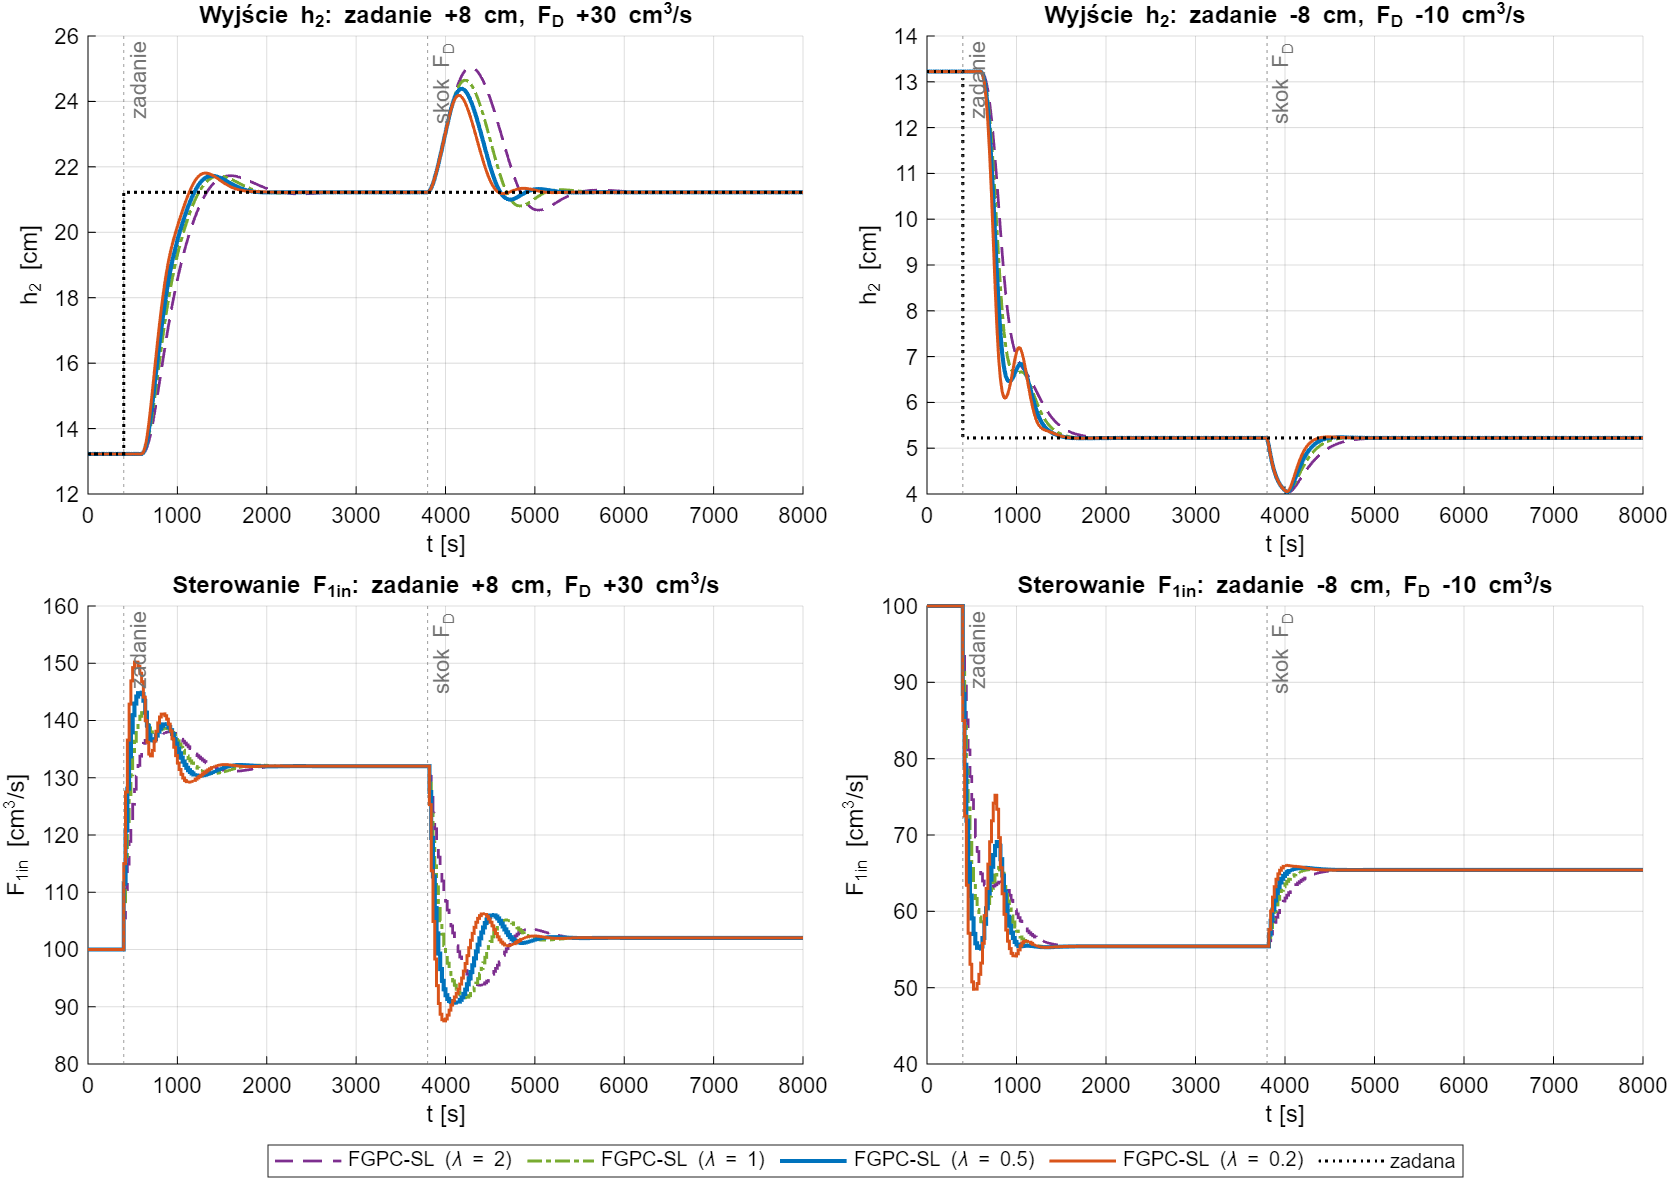
\includegraphics[width=\textwidth]{rysunki/czesc3/strojenie_SL.png}
\caption{Wpływ parametru $\lambda$ w regulatorze FGPC--SL (${N=30}$, ${N_u=5}$) w skrajnych próbach $+8\ \mathrm{cm}$ / $+30\ \jednprzep$ oraz $-8\ \mathrm{cm}$ / $-10\ \jednprzep$.}
\label{fig:sl-tuning}
\end{figure}
\begin{figure}[H]
\centering
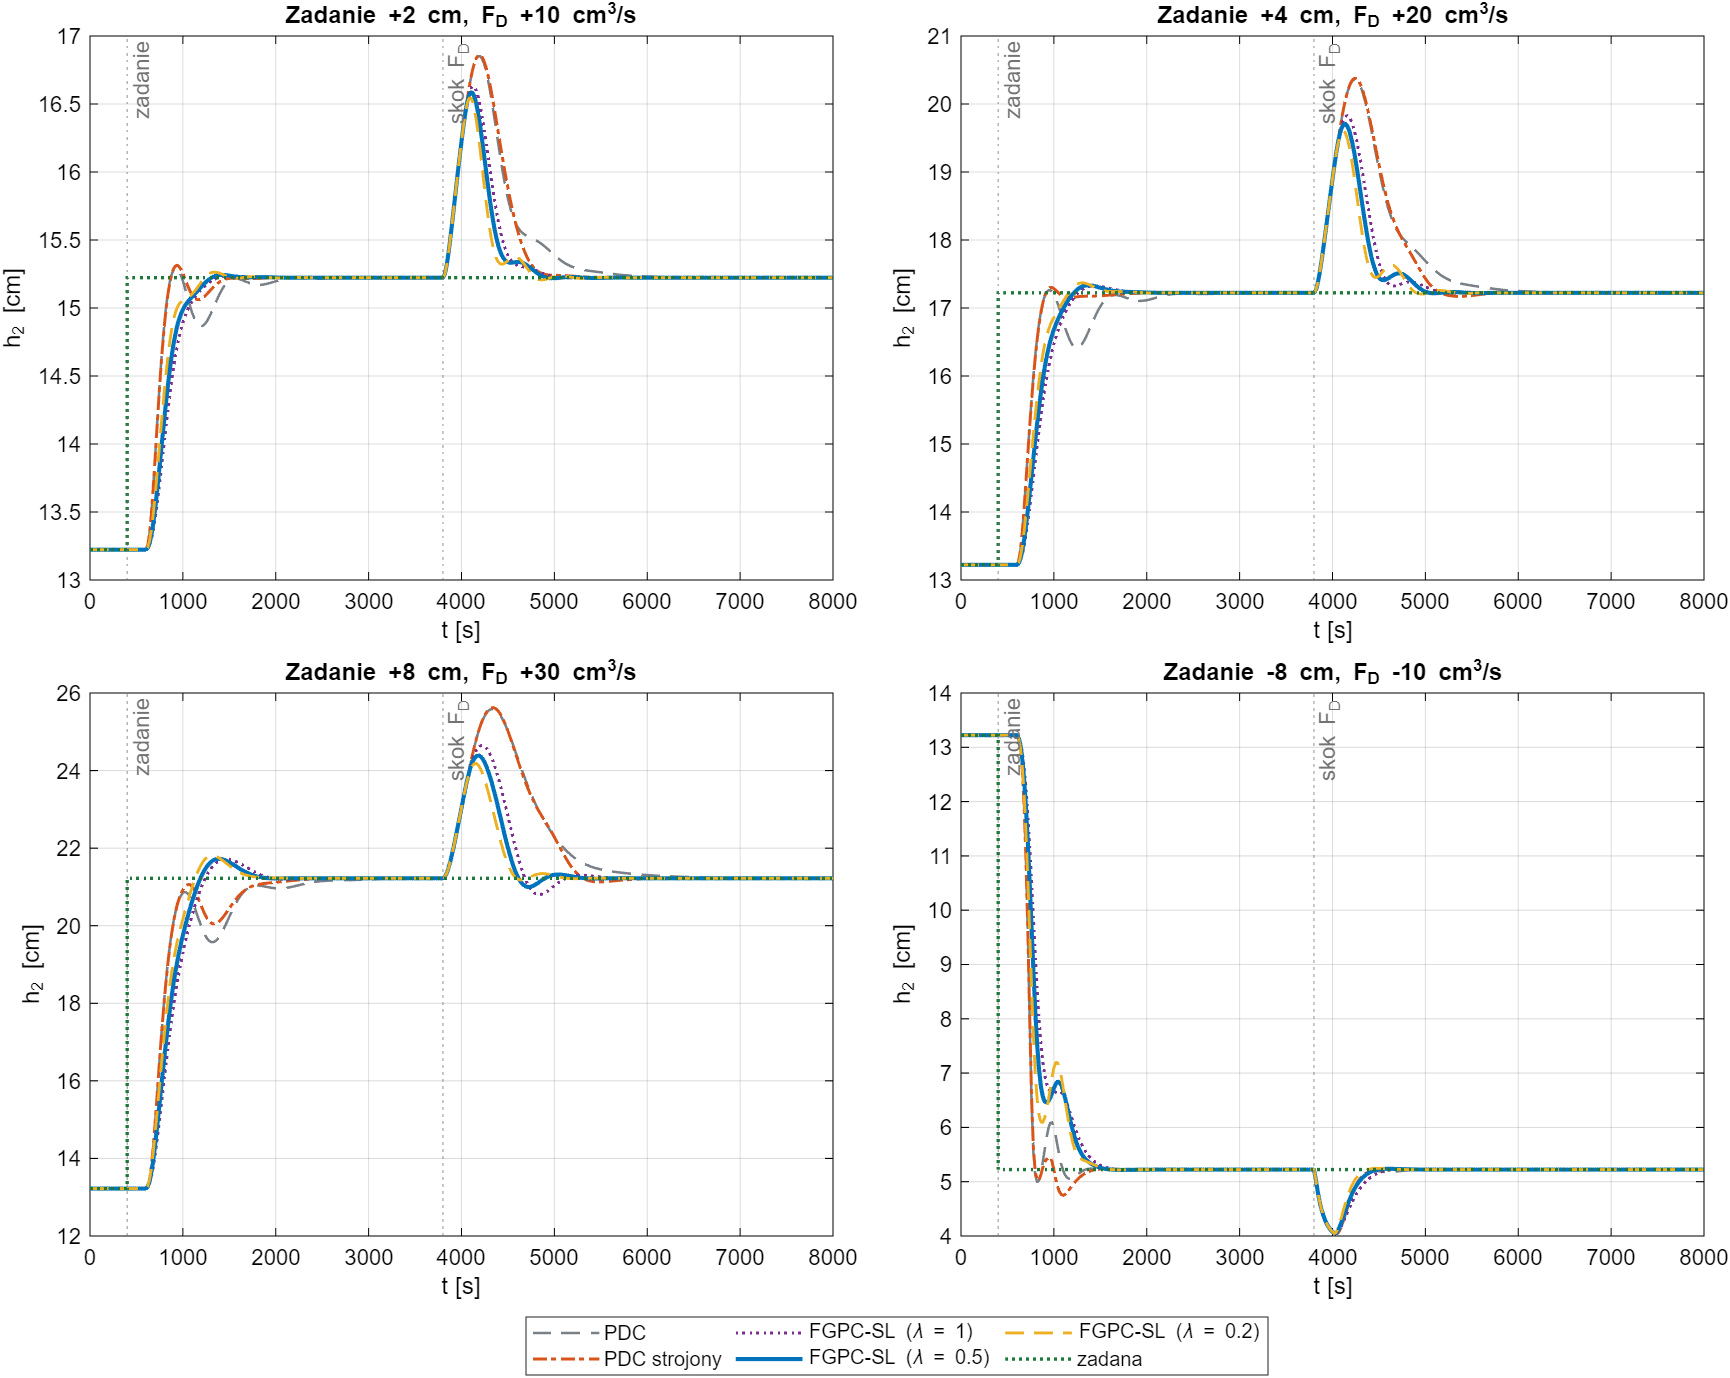
\includegraphics[width=\textwidth]{rysunki/czesc3/porownanie_wyjsc.png}
\caption{Poziom $h_2$ w czterech próbach projektowych: PDC, PDC strojony oraz FGPC--SL (${\lambda=1}$, ${\lambda=\num{0.5}}$ i ${\lambda=\num{0.2}}$).}
\label{fig:sl-outputs}
\end{figure}
\begin{figure}[H]
\centering
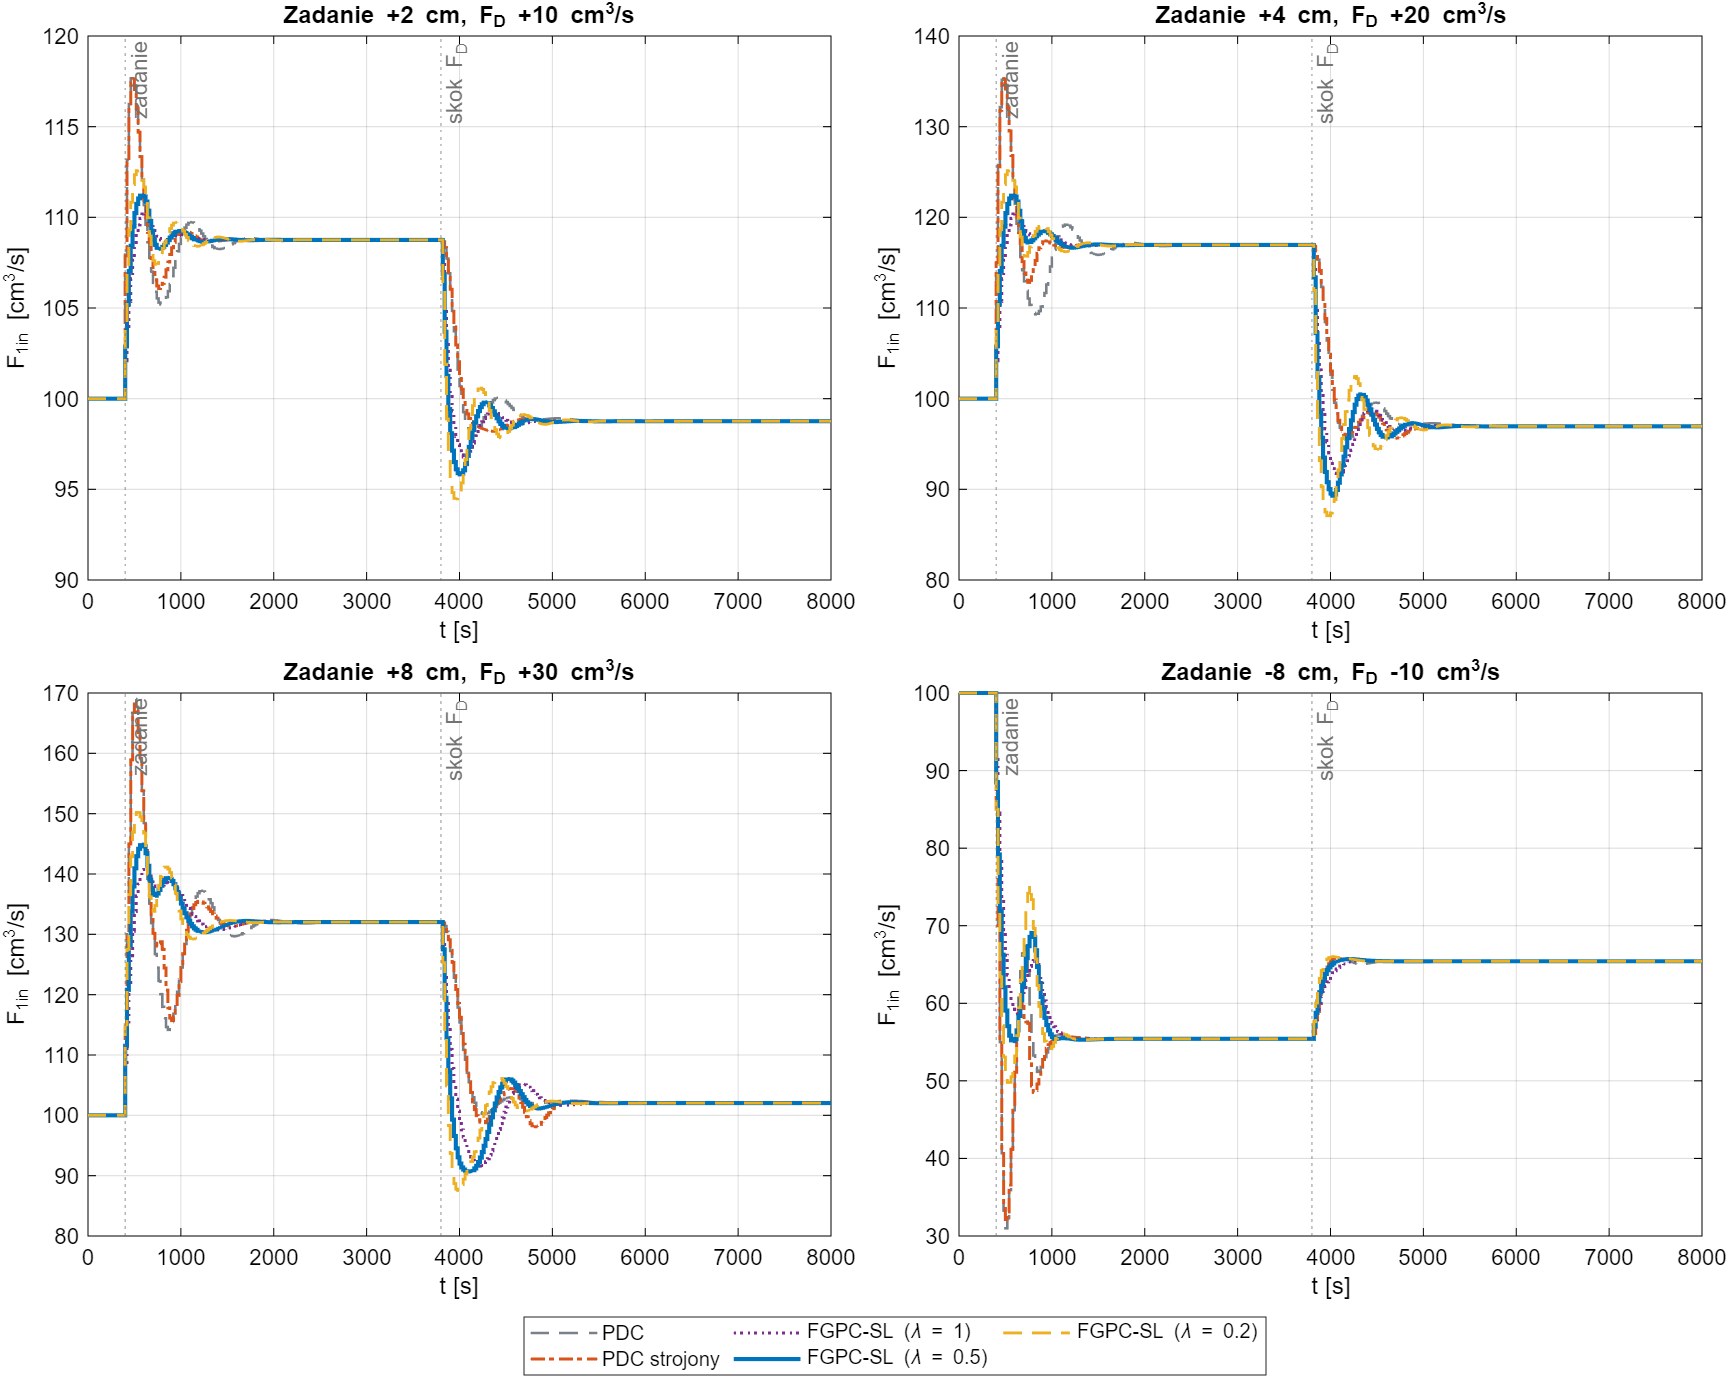
\includegraphics[width=\textwidth]{rysunki/czesc3/porownanie_sterowan.png}
\caption{Dopływ sterujący $\uvar$ dla przebiegów z rys.~\ref{fig:sl-outputs}.}
\label{fig:sl-controls}
\end{figure}
